\documentclass[11pt]{article}
\usepackage{amsmath, amssymb, amsfonts, amsthm}
\usepackage{geometry}
\geometry{letterpaper, margin=0.5in}
\usepackage{booktabs}
\usepackage{tikz}

\theoremstyle{definition} 
\newtheorem{definition}{Definition}[section] % [section] resets numbering per section

\newcommand{\NameText}{\texttt{SU(n=5, q=2, eps=1)}}
\newcommand{\MatrixSize}{5}
\newcommand{\Rank}{2}

\title{Pinned group summary: \NameText{}}
\author{Pinning-Sympy automated output}
\date{\today}

\begin{document}

\maketitle
\tableofcontents

\newpage

\section{Basic attributes}

\begin{tabular}{|l|l|}
	\hline
    Group & \NameText \\
	\hline
    Matrix size & $\MatrixSize \times \MatrixSize$ \\
	\hline
    Rank & $\Rank$ \\
	\hline
\end{tabular}

\subsection{Hermitian form}
\begin{tabular}{|l|l|}
    \hline
    Dimension & 5 \\
    \hline
    Witt index & 2 \\
    \hline
    Primitive element & $\sqrt{d}$ \\
    \hline
    Epsilon & $1$ \\
    \hline
\end{tabular}

\bigskip
\noindent Matrix: \(
\left[\begin{matrix}0 & 0 & 1 & 0 & 0\\0 & 0 & 0 & 1 & 0\\1 & 0 & 0 & 0 & 0\\0 & 1 & 0 & 0 & 0\\0 & 0 & 0 & 0 & c_{0}\end{matrix}\right]
\)



\subsection{Generic Lie algebra element}
\[
\left[\begin{matrix}\sqrt{d} x_{i 0 0} + x_{r 0 0} & \sqrt{d} x_{i 0 1} + x_{r 0 1} & \sqrt{d} x_{i 0 2} & \sqrt{d} x_{i 1 2} - x_{r 1 2} & - c_{0} \left(- \sqrt{d} x_{i 4 2} + x_{r 4 2}\right)\\\sqrt{d} x_{i 1 0} + x_{r 1 0} & - \sqrt{d} x_{i 0 0} - \frac{\sqrt{d} x_{i 4 4}}{2} + x_{r 1 1} & \sqrt{d} x_{i 1 2} + x_{r 1 2} & \sqrt{d} x_{i 1 3} & - c_{0} \left(- \sqrt{d} x_{i 4 3} + x_{r 4 3}\right)\\\sqrt{d} x_{i 2 0} & \sqrt{d} x_{i 3 0} - x_{r 3 0} & \sqrt{d} x_{i 0 0} - x_{r 0 0} & \sqrt{d} x_{i 1 0} - x_{r 1 0} & - c_{0} \left(- \sqrt{d} x_{i 4 0} + x_{r 4 0}\right)\\\sqrt{d} x_{i 3 0} + x_{r 3 0} & \sqrt{d} x_{i 3 1} & \sqrt{d} x_{i 0 1} - x_{r 0 1} & - \sqrt{d} x_{i 0 0} - \frac{\sqrt{d} x_{i 4 4}}{2} - x_{r 1 1} & - c_{0} \left(- \sqrt{d} x_{i 4 1} + x_{r 4 1}\right)\\\sqrt{d} x_{i 4 0} + x_{r 4 0} & \sqrt{d} x_{i 4 1} + x_{r 4 1} & \sqrt{d} x_{i 4 2} + x_{r 4 2} & \sqrt{d} x_{i 4 3} + x_{r 4 3} & \sqrt{d} x_{i 4 4}\end{matrix}\right]
\]

\subsection{Generic torus element}
\[
\left[\begin{matrix}t_{0} & 0 & 0 & 0 & 0\\0 & t_{1} & 0 & 0 & 0\\0 & 0 & \frac{1}{t_{0}} & 0 & 0\\0 & 0 & 0 & \frac{1}{t_{1}} & 0\\0 & 0 & 0 & 0 & 1\end{matrix}\right]
\]

\subsection{Trivial characters}
\[
\left[\begin{matrix}1 & 0 & 1 & 0 & 0\\0 & 1 & 0 & 1 & 0\\1 & 1 & 1 & 1 & 1\end{matrix}\right]
\]

\newpage
\section{Root system}

\subsection*{Summary Properties}
\begin{tabular}{|l|l|}
    \hline
    Dynkin type & \texttt{BC2} \\
    \hline
    Reduced & False \\
    \hline
    Simply laced & False \\
    \hline
    Number of roots & 12 \\
    \hline
\end{tabular}

\subsection{Dynkin diagram}
\begin{center}
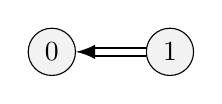
\begin{tikzpicture}[
    node/.style={circle, draw, fill=black!5, minimum size=6mm, inner sep=0pt},
    arrow/.style={-latex, thick},
    doublearrow/.style={double, double distance=2pt, -latex, thick},
    triplearrow/.style={double, double distance=4pt, -latex, thick},
    plain/.style={thick},
    baseline=(current bounding box.center)
]
    \node[node] (0) at (0.00, 0.00) {$0$};
    \node[node] (1) at (1.50, 0.00) {$1$};
    \draw[doublearrow] (1) -- (0);
\end{tikzpicture}
\end{center}

\subsection{Cartan matrix}
\[
\left[\begin{matrix}2 & -1\\-2 & 2\end{matrix}\right]
\]

\subsection{Roots and coroots}
\begin{center}
\begin{tabular}{|l|l|c|c|c|}
    \hline
    \textbf{Root} & \textbf{Coroot} & \textbf{Simple} & \textbf{Sign} & \textbf{Multipliable} \\
    \hline
    $\left( -2, \  0, \  0, \  0, \  0\right)$ & $\left( -1, \  0, \  1, \  0, \  0\right)$ & No & $-$ & No \\
    \hline
    $\left( -1, \  -1, \  0, \  0, \  0\right)$ & $\left( -1, \  -1, \  1, \  1, \  0\right)$ & No & $-$ & No \\
    \hline
    $\left( -1, \  0, \  0, \  0, \  0\right)$ & $\left( -2, \  0, \  2, \  0, \  0\right)$ & No & $-$ & Yes \\
    \hline
    $\left( -1, \  1, \  0, \  0, \  0\right)$ & $\left( -1, \  1, \  1, \  -1, \  0\right)$ & No & $-$ & No \\
    \hline
    $\left( 0, \  -2, \  0, \  0, \  0\right)$ & $\left( 0, \  -1, \  0, \  1, \  0\right)$ & No & $-$ & No \\
    \hline
    $\left( 0, \  -1, \  0, \  0, \  0\right)$ & $\left( 0, \  -2, \  0, \  2, \  0\right)$ & No & $-$ & Yes \\
    \hline
    $\left( 0, \  1, \  0, \  0, \  0\right)$ & $\left( 0, \  2, \  0, \  -2, \  0\right)$ & Yes & $+$ & Yes \\
    \hline
    $\left( 0, \  2, \  0, \  0, \  0\right)$ & $\left( 0, \  1, \  0, \  -1, \  0\right)$ & No & $+$ & No \\
    \hline
    $\left( 1, \  -1, \  0, \  0, \  0\right)$ & $\left( 1, \  -1, \  -1, \  1, \  0\right)$ & Yes & $+$ & No \\
    \hline
    $\left( 1, \  0, \  0, \  0, \  0\right)$ & $\left( 2, \  0, \  -2, \  0, \  0\right)$ & No & $+$ & Yes \\
    \hline
    $\left( 1, \  1, \  0, \  0, \  0\right)$ & $\left( 1, \  1, \  -1, \  -1, \  0\right)$ & No & $+$ & No \\
    \hline
    $\left( 2, \  0, \  0, \  0, \  0\right)$ & $\left( 1, \  0, \  -1, \  0, \  0\right)$ & No & $+$ & No \\
    \hline
\end{tabular}
\end{center}


\subsection{Linear combinations of roots}

\begin{definition}
For two roots $\alpha, \beta$ in a root system $\Phi$, the set of positive integral linear combinations of $\alpha, \beta$ that are also roots is denoted
\[
	(\alpha, \beta) = \{ i \alpha + j \beta \in \Phi : i, j \in \mathbb{Z}_{\ge 1} \}
\]
\end{definition}

\begin{center}
\begin{tabular}{|l|l|c|}
    \hline
    $\alpha$ & $\beta$ & Pairs $(i,j)$ \\
    \hline
    $\left( -2, \  0, \  0, \  0, \  0\right)$ & $\left( 1, \  -1, \  0, \  0, \  0\right)$ & $(1,1), (1,2)$ \\
    \hline
    $\left( -2, \  0, \  0, \  0, \  0\right)$ & $\left( 1, \  0, \  0, \  0, \  0\right)$ & $(1,1)$ \\
    \hline
    $\left( -2, \  0, \  0, \  0, \  0\right)$ & $\left( 1, \  1, \  0, \  0, \  0\right)$ & $(1,1), (1,2)$ \\
    \hline
    $\left( -1, \  -1, \  0, \  0, \  0\right)$ & $\left( -1, \  1, \  0, \  0, \  0\right)$ & $(1,1)$ \\
    \hline
    $\left( -1, \  -1, \  0, \  0, \  0\right)$ & $\left( 0, \  1, \  0, \  0, \  0\right)$ & $(1,1), (1,2), (2,2)$ \\
    \hline
    $\left( -1, \  -1, \  0, \  0, \  0\right)$ & $\left( 0, \  2, \  0, \  0, \  0\right)$ & $(1,1), (2,1)$ \\
    \hline
    $\left( -1, \  -1, \  0, \  0, \  0\right)$ & $\left( 1, \  -1, \  0, \  0, \  0\right)$ & $(1,1)$ \\
    \hline
    $\left( -1, \  -1, \  0, \  0, \  0\right)$ & $\left( 1, \  0, \  0, \  0, \  0\right)$ & $(1,1), (1,2), (2,2)$ \\
    \hline
    $\left( -1, \  -1, \  0, \  0, \  0\right)$ & $\left( 2, \  0, \  0, \  0, \  0\right)$ & $(1,1), (2,1)$ \\
    \hline
    $\left( -1, \  0, \  0, \  0, \  0\right)$ & $\left( 0, \  -1, \  0, \  0, \  0\right)$ & $(1,1)$ \\
    \hline
    $\left( -1, \  0, \  0, \  0, \  0\right)$ & $\left( 0, \  1, \  0, \  0, \  0\right)$ & $(1,1)$ \\
    \hline
    $\left( -1, \  0, \  0, \  0, \  0\right)$ & $\left( 1, \  -1, \  0, \  0, \  0\right)$ & $(1,1), (2,1), (2,2)$ \\
    \hline
    $\left( -1, \  0, \  0, \  0, \  0\right)$ & $\left( 1, \  1, \  0, \  0, \  0\right)$ & $(1,1), (2,1), (2,2)$ \\
    \hline
    $\left( -1, \  0, \  0, \  0, \  0\right)$ & $\left( 2, \  0, \  0, \  0, \  0\right)$ & $(1,1)$ \\
    \hline
    $\left( -1, \  1, \  0, \  0, \  0\right)$ & $\left( 0, \  -2, \  0, \  0, \  0\right)$ & $(1,1), (2,1)$ \\
    \hline
    $\left( -1, \  1, \  0, \  0, \  0\right)$ & $\left( 0, \  -1, \  0, \  0, \  0\right)$ & $(1,1), (1,2), (2,2)$ \\
    \hline
    $\left( -1, \  1, \  0, \  0, \  0\right)$ & $\left( 1, \  0, \  0, \  0, \  0\right)$ & $(1,1), (1,2), (2,2)$ \\
    \hline
    $\left( -1, \  1, \  0, \  0, \  0\right)$ & $\left( 1, \  1, \  0, \  0, \  0\right)$ & $(1,1)$ \\
    \hline
    $\left( -1, \  1, \  0, \  0, \  0\right)$ & $\left( 2, \  0, \  0, \  0, \  0\right)$ & $(1,1), (2,1)$ \\
    \hline
    $\left( 0, \  -2, \  0, \  0, \  0\right)$ & $\left( 0, \  1, \  0, \  0, \  0\right)$ & $(1,1)$ \\
    \hline
    $\left( 0, \  -2, \  0, \  0, \  0\right)$ & $\left( 1, \  1, \  0, \  0, \  0\right)$ & $(1,1), (1,2)$ \\
    \hline
    $\left( 0, \  -1, \  0, \  0, \  0\right)$ & $\left( 0, \  2, \  0, \  0, \  0\right)$ & $(1,1)$ \\
    \hline
    $\left( 0, \  -1, \  0, \  0, \  0\right)$ & $\left( 1, \  0, \  0, \  0, \  0\right)$ & $(1,1)$ \\
    \hline
    $\left( 0, \  -1, \  0, \  0, \  0\right)$ & $\left( 1, \  1, \  0, \  0, \  0\right)$ & $(1,1), (2,1), (2,2)$ \\
    \hline
    $\left( 0, \  1, \  0, \  0, \  0\right)$ & $\left( 1, \  -1, \  0, \  0, \  0\right)$ & $(1,1), (2,1), (2,2)$ \\
    \hline
    $\left( 0, \  1, \  0, \  0, \  0\right)$ & $\left( 1, \  0, \  0, \  0, \  0\right)$ & $(1,1)$ \\
    \hline
    $\left( 0, \  2, \  0, \  0, \  0\right)$ & $\left( 1, \  -1, \  0, \  0, \  0\right)$ & $(1,1), (1,2)$ \\
    \hline
    $\left( 1, \  -1, \  0, \  0, \  0\right)$ & $\left( 1, \  1, \  0, \  0, \  0\right)$ & $(1,1)$ \\
    \hline
\end{tabular}
\end{center}


\end{document}